\documentclass{article}
\usepackage{hyperref}
\usepackage{amsmath}
\usepackage{amssymb}
\usepackage{pgfplots}
\usepackage{float}
\usepackage{todonotes}
\usepackage{tikz}
\usepackage[shortlabels]{enumitem}

\renewcommand{\Re}{\mathbb{R}}
\newcommand{\Li}{\mathcal{L}}
\newcommand{\Ex}{\mathbb{E}}
\renewcommand{\Pr}{\mathbb{P}}
\newcommand{\Hy}{\mathcal{H}}
\newcommand{\sign}{\text{sign}}
\newcommand{\error}{\text{error}}

\newcommand\bigO[1]{
    \ensuremath{\mathcal{O}\left(#1\right)}
    }

\newcommand{\sigmoidPlot}{
    
    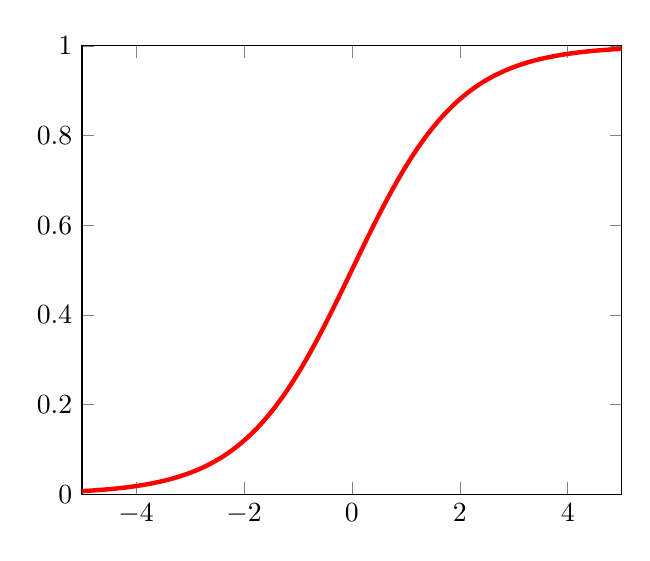
\begin{tikzpicture}
        \begin{axis}[xmin=-5, xmax=5, ymin=0, ymax=1, samples=150]
        \addplot[red, ultra thick] {1/(1+exp(-x))};
        \end{axis}
    \end{tikzpicture}
    
    }

\usetikzlibrary{positioning, calc}
\usetikzlibrary{arrows.meta}

\tikzstyle{circlebox}=[circle,thick,draw=black!75,minimum size=8mm]
\tikzstyle{inputnode}=[circlebox, draw=blue!75]
\tikzstyle{hiddennode}=[circlebox, draw=orange!75]
\tikzstyle{outputnode}=[circlebox, draw=orange!75]
\tikzstyle{simplebox}=[rectangle,thick,draw=black!75,
fill=black!20,minimum size=4mm]
\tikzstyle{textbox}=[rectangle,thick,minimum size=4mm,draw=black!0,
fill=black!0]
\tikzstyle{halfvdistance}=[yshift=-0.7cm]
\tikzstyle{abovebetween}=[xshift=-2.7mm]
\tikzstyle{edgepath} = [-Latex,->,shorten >=1pt,-stealth,semithick, rounded 
corners=5pt]

\def \nodedv {0.735cm}
\def \nodedh {0.65cm}

\tikzset{
    between/.style args={#1 and #2}{
        at = ($(#1)!0.5!(#2)$)
    }
}

\begin{document}
    \section{Subjects}
    \begin{itemize}
        \item Kernels
    \end{itemize}
    \section{Notes}
    
    \url{https://www.youtube.com/watch?v=_PwhiWxHK8o}
    
    \subsection{Decision boundaries}
    Instead of just finding a hyperplane that separates the data, we want to 
    find the (median) line that leaves as much space as possible between the 
    two classes of data. This line has a gutter on both sides of the boundary, 
    which intersects the closes point on each side. The gutter and the median 
    line are all parallel and one can think of them as a broad road.
    
    \subsubsection{The decision rule}
    Suppose we have some vector $w$ which is perpendicular to the median line, 
    we can then say that if:
    \begin{equation*}
        w \cdot u \geq C
    \end{equation*}
    then the unknown vector $u$ is on ``the positive side'' of the decision 
    boundary and thus should have a positive label. We can rewrite this as:
    \begin{equation*}
        w \cdot u + b \geq 0 \text{ then +}, \quad C = -b
    \end{equation*}
    and this constitutes our decision rule.\\
    Now we want to find $b$ and $w$ such that the following two equations to 
    hold:
    \begin{align*}
        w \cdot x_i + b \geq 1, \qquad &\text{if } y_i = 1\\
        w \cdot x_i + b \leq -1, \qquad &\text{if } y_i = -1
    \end{align*}
    
    We can simplify that as:
    \begin{align*}
        y_i (w \cdot x_i + b) &\geq 1\\
        \Downarrow\\
        y_i (w \cdot x_i + b) - 1 &\geq 0
    \end{align*}
    
    Furthermore we want the following equation to hold for points in the gutter:
    \begin{equation*}
        y_i (w \cdot x_i + b) - 1 = 0
    \end{equation*}
    
    \subsubsection{The distance between the gutters}
    Suppose we have two vectors, $x_+$ which points to an $x_i$ for which $y_i 
    = 1$ and $x_-$ which points to an $x_i$ for which $y_i = -1$.
    
    Now, if we had a unit vector which was perpendicular to one of the gutters, 
    then we could just dot the difference vector $x_+-x_-$ with the unit vector 
    and that would be the width.
    
    However, earlier we said that $w$ was exactly perpendicular to the median 
    line, then we can define the width of the road as:
    \begin{equation*}
        \text{width} = (x_+-x_-) \cdot \frac{w}{\|w\|}
    \end{equation*}
    Now, recall that:
    \begin{equation*}
        y_i (w \cdot x_i + b) - 1 = 0
    \end{equation*}
    for some $x_i$ in the gutter. We can isolate $x_i \cdot w$ and get:
    \begin{equation*}
        w \cdot x_i = 1-y_ib
    \end{equation*}
    And we can rewrite the width as:
    \begin{align*}
        \text{width} &= \frac{x_+ \cdot w}{\|w\|} - \frac{x_- \cdot w}{\|w\|}\\
            &= \frac{1 - b}{\|w\|} - \frac{1 + b}{\|w\|}\\
            &= \frac{2}{\|w\|}
    \end{align*}
    And what we are trying to achieve, is finding the widest street between the 
    two sets, so this gives us exactly what we are trying to maximize. So we 
    will be trying to maximize $\frac{2}{\|w\|}$ which is the same as 
    minimizing $\|w\|$.
    
    For mathematical convenience, we will try to minimize $\frac{1}{2}\|w\|^2$ 
    instead.
    
    To summarize, given that $w$ is perpendicular to the road we have the 
    following expression that we want to minimize in order to maximize the 
    width of the road:
    \begin{equation*}
        \frac{1}{2}\|w\|^2
    \end{equation*} 
    And we want to satisfy the following two constraints:
    \begin{align*}
        y_i (w \cdot x_i + b) - 1 &\geq 0\\
        y_i (w \cdot x_i + b) - 1 &=0, \quad \text{ íf $x_i$ is in the gutter}
    \end{align*}
    
    We can then use lagrange multipliers in order to find the extremum of the 
    function:
    \begin{equation*}
        L = \frac{1}{2} \|w\|^2 - \sum_{i=1}^{N} \alpha_i \left[y_i(w \cdot x_i 
        + 
        b) - 1\right]
    \end{equation*}
    Then we need to find the derivatives and set them to $0$
    \begin{align*}
        \frac{\partial L}{\partial w} &= w - \sum_{i=1}^{N} \alpha_i y_i x_i = 
        0\\
        w &= \sum_{i=1}^{N}\alpha_i y_i x_i
    \end{align*}
    This means that we can express $w$ as the linear combination of some of the 
    points in the data-set multiplied by their labels ($-1$ or $+1$) and some 
    $\alpha_i$ which will be $0$ for some of them.
    
    \begin{align*}
    \frac{\partial L}{\partial b} &= -\sum_{i=1}^{N} \alpha_i y_i = 0 \implies 
    \sum_{i=1}^{N} \alpha_i y_i = 0
    \end{align*}
    
    We can now plug the definition of $w$ back into the expression of $L$:
    
    \begin{align*}
    L &= \frac{1}{2} \|w\|^2 - \sum_{i=1}^{N} \alpha_i y_i(w \cdot x_i + 
    b) - \alpha_i\\
    L &= \frac{1}{2} \|w\|^2 - \sum_{i=1}^{N} \alpha_i y_i (w \cdot x_i) + 
    \alpha_i y_i b - \alpha_i\\
    L &= \frac{1}{2} \left(\sum_{i=1}^{N}\alpha_i y_i x_i\right) \cdot 
    \left(\sum_{i=1}^{N}\alpha_i y_i x_i\right) - 
    \left(\sum_{i=1}^{N} \alpha_i y_i x_i \cdot \left(\sum_{j=1}^{N}\alpha_j 
    y_j x_j\right)\right)
    - \sum_{i=1}^{N} \alpha_i y_i b 
    + \sum_{i=1}^{N} \alpha_i\\
    L &= \frac{1}{2} \left(\sum_{i=1}^{N}\alpha_i y_i x_i\right) \cdot 
    \left(\sum_{i=1}^{N}\alpha_i y_i x_i\right) - 
    \left(\sum_{i=1}^{N} \alpha_i y_i x_i \cdot \left(\sum_{j=1}^{N}\alpha_j 
    y_j x_j\right)\right)
    - b\sum_{i=1}^{N} \alpha_i y_i
    + \sum_{i=1}^{N} \alpha_i
    + \sum_{i=1}^{N} \alpha_i\\
    L &= \frac{1}{2} \left(\sum_{i=1}^{N}\alpha_i y_i x_i\right) \cdot 
    \left(\sum_{i=1}^{N}\alpha_i y_i x_i\right) - 
    \left(\sum_{i=1}^{N} \alpha_i y_i x_i \cdot \left(\sum_{j=1}^{N}\alpha_j 
    y_j x_j\right)\right)
    + \sum_{i=1}^{N} \alpha_i\\
    L &= \frac{1}{2} \left(\sum_{i=1}^{N}\alpha_i y_i x_i\right) \cdot 
    \left(\sum_{i=1}^{N}\alpha_i y_i x_i\right) - 
    \left(\sum_{i=1}^{N} \alpha_i y_i x_i \right) \cdot 
    \left(\sum_{j=1}^{N}\alpha_j y_j x_j\right)
    + \sum_{i=1}^{N} \alpha_i\\
    L &= \sum_{i=1}^{N} \alpha_i - 
    \frac{1}{2} \left(\sum_{i=1}^{N} \sum_{j=1}^{N} \alpha_i\alpha_j y_iy_j 
    x_i \cdot x_j \right)
    \end{align*}
    
    Furthermore, we can insert $w$ into the decision rule as well:
    \begin{equation*}
        \left(\sum_{i=1}^{N} \alpha_i y_i x_i \cdot u\right) + b \geq 0 \quad 
        \text{ then +}
    \end{equation*}
    \todo{How do we then find $\alpha_i$?}
    
    Most of the $\alpha_i$'s will be $0$, thus we only have to compute the dot 
    product of a very small amount of pairs of $x_i$ and $u$. The points that 
    have $\alpha_i=0$ is the points that we call the support vectors. This is 
    what makes SVM efficient, even in very high dimensional spaces.
    
    \subsubsection{Kernels}
    Instead of taking the dot-product of $x_i$ and $u$, we can replace it with 
    a kernel $K$ which takes non-linear data and outputs linear-data. And thus 
    it is able to compute the SVM for even non-linear data!
    
    We can represent a feature mapping as $\phi(x) \cdot \phi(z)$ and then the 
    kernel will be:
    \begin{equation*}
        K(x,z) = \phi(x)^T\phi(z)
    \end{equation*}
    However, often there can be found more efficient ways to compute $K(x,z)$ 
    than computing and representing the $\phi$ vectors, if we choose to compute 
    $K(x,z)$ directly.
    
    \subsubsection{Regularization and the non-separable case}
    Luckily, regularization and the non-separable case go hand-in-hand as 
    regularizing also helps the non-separable case. We simply reformulate our 
    optimization as follows:
    \begin{align*}
        \text{minimize: }&\frac{1}{2}\|w\|^2 + C \sum_{i=1}^{N}\xi_i\\
        \text{s.t.: }&y_i(w \cdot x_i + b) \geq 1-\xi_i, \quad i=1,\dots,N
    \end{align*}
    
    
\end{document}